\documentclass[a4j]{jarticle}
\usepackage[dvipdfmx]{graphicx}
\usepackage{subfig}

\renewcommand{\labelenumi}{(\arabic{enumi})}

\title{中間報告書(1) \\ A班}
\author{秋元淳矢 \and 天笠智哉 \and 小林広人}
\date{}

\begin{document}

\maketitle

\section{現在の状況}
\subsection{完成した機能}
現在、完成している機能を以下に示す。
\begin{description}
	\item[WishListのModel] \mbox{} \\
		WishListのModel \\
		WishListのModel
	\item[Menu] \mbox{} \\
    	図\ref{MenuFig1}にAndroidの環境でmenuを表示したときの画面示す。
		画面左端からのスワイプで表示されるMenuをMasterDetailPageを使うことで実装した。
        Menuの項目はCalendar,ToDo,WishList,家計簿の4つで、項目を押すとそれぞれの画面に遷移する。
        
        \begin{figure}[h]
			\centering
 			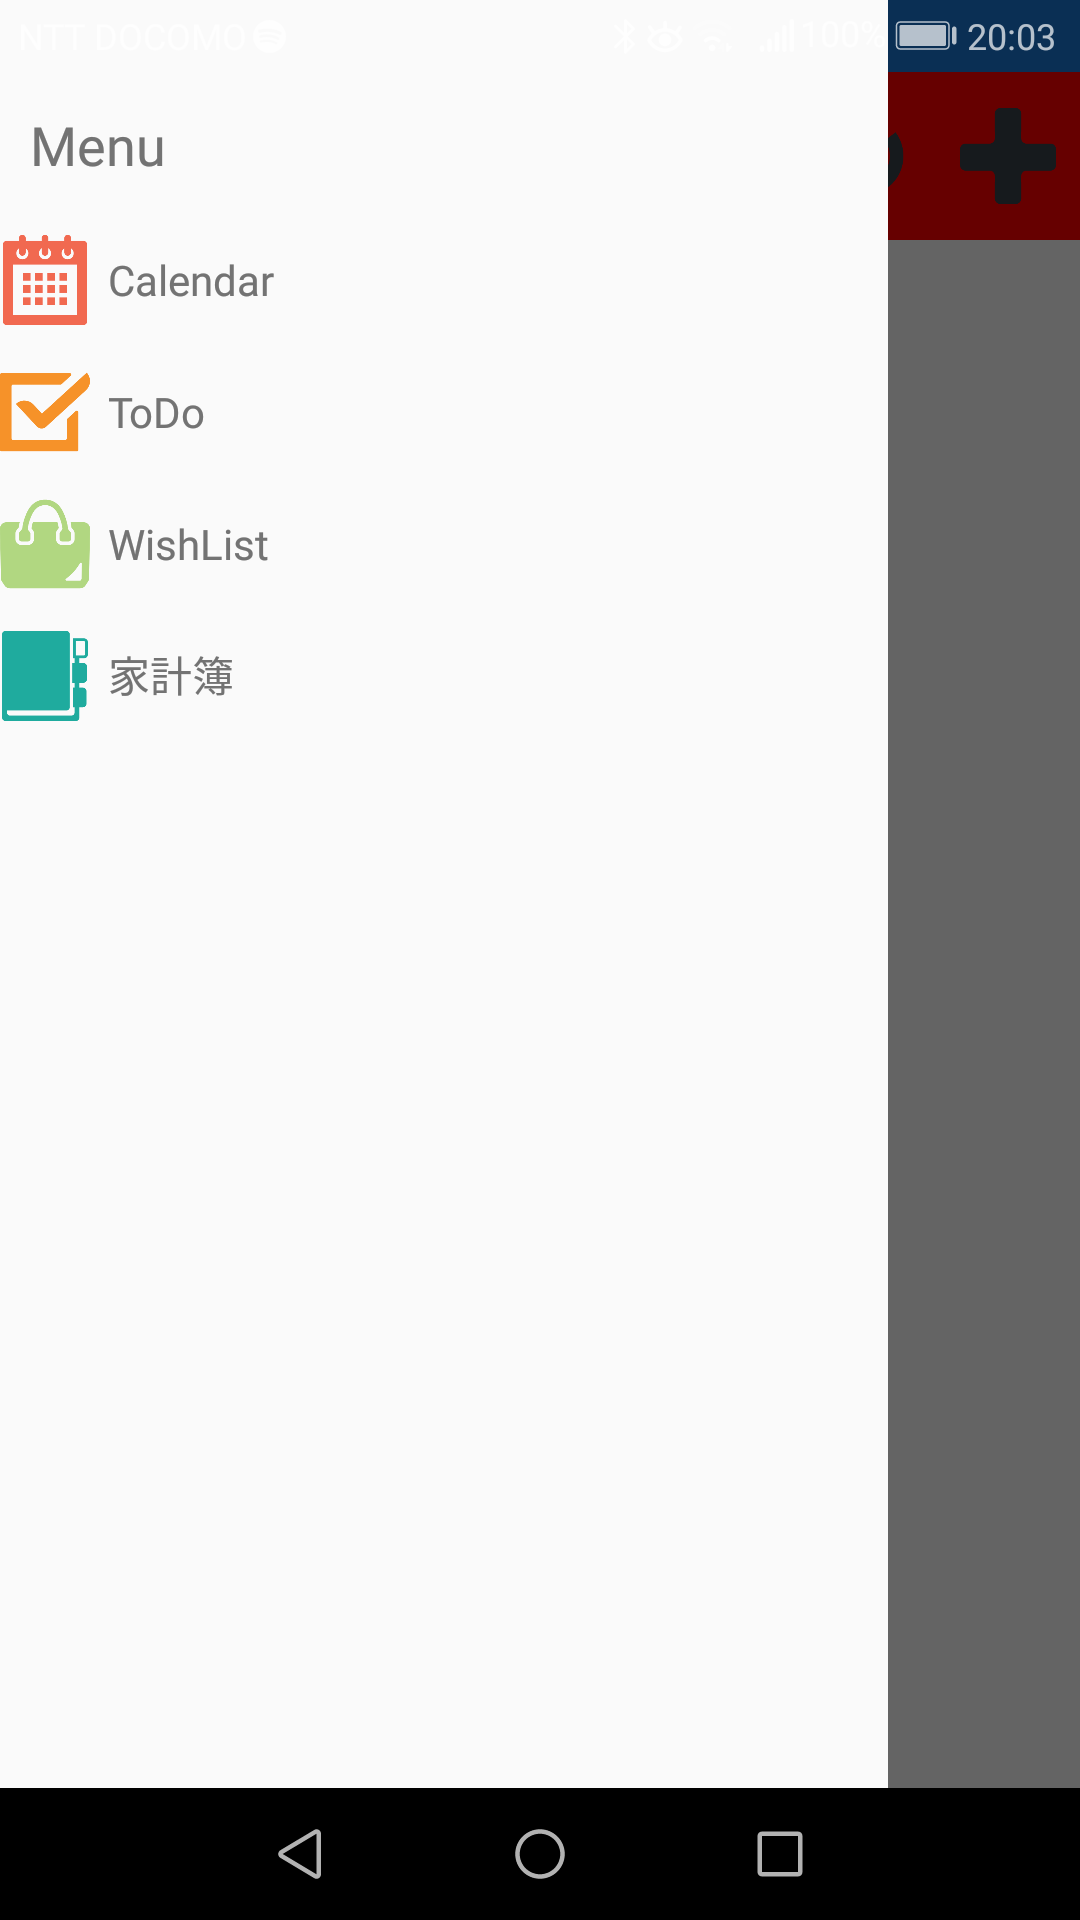
\includegraphics[width=80mm]{figures/MenuPage.png} %パスをかえる
 			\caption{Androidの環境でmenuを表示したときの画面図}
 			\label{MenuFig1} %Nの部分をかえる
		\end{figure}
\end{description}


\subsection{開発中の機能}
現在開発中の機能を以下に示す。
\begin{description}
	\item[CalenderのModel] \mbox{} \\
		CalenderのModel
\end{description}


\section{今後の課題}



\section{補足}
仕様書の説明が不十分である点が数か所見受けられた。
以下に追加する補足説明を示す。


\end{document}
